\chapter{Construction and Manufacturing} \label{chapter3}

\section{Base material} \label{bmaterial}

To accurately describe the expected dimensions of this base material it is important to know the target PCB size for the concerned CNC machine since along with the required machinery and hardware that would be mounted on the base material, the PCB is the main working component. For this project the designers have targeted $\boldsymbol{15}$ \textbf{cm} $\boldsymbol{\times}$ $\boldsymbol{15}$ \textbf{cm single sided copper clad PCBs}. \par

It is obvious that the net dimensions of the base material would need to be greater than that of the target PCB size. After performing multiple calculations as described in the following sections. The final base material size has been fixed at $\boldsymbol{40}$ \textbf{cm} $\boldsymbol{\times}$ $\boldsymbol{40}$ \textbf{cm} .

\begin{figure}[h]
 \centering
 \begin{tikzpicture}[scale=0.2]
  \draw (0,0) rectangle (40,40);
  \draw [blue] (0,0) rectangle (15,15);
 \end{tikzpicture}
 \caption{Drawing showing maximum PCB dimensions that can be manufactured (in \textcolor{blue}{blue}) superimposed on base material dimensions represented on a $1:5$ scale}
 \label{fig:base}
\end{figure}


\section{XY axes made up of normal unpolished wood}

The two segments of wood which must have the primary load bearing capacity are the XY axes. The X segment consists of a wooden plank like structure with slots of length $15$ mm and depth $8$ mm each to insert wooden blocks on it. A similar structure exists for Y - axis segment as well. Dimensions for both the segments are illustrated below. \par 


\begin{figure}[h]
 \begin{center}
  \begin{tikzpicture}[scale=0.2]
   \draw (0,0) rectangle (8.5,40);
   \draw [dashed] (0,1.7) rectangle (8.5,1.7);
   \draw [dashed] (0,3.2) rectangle (8.5,3.2);
   \draw [dashed] (0,28.5) rectangle (8.5,28.5);
   \draw [dashed] (0,30) rectangle (8.5,30);
   \hspace{-15mm}
   \dimline [extension start length=0.25, extension end length=0.25, line style = {line width=0.5}]{(0,0)}{(0,40)}{40 cm};
   \hspace{15mm}
   \dimline[line style={line width=0.5},extension start length=1,extension end length=1]{(0,42)}{(8.5,42)}{8.5 cm};
   \dimline[line style={line width=0.5},extension start length=0.3,extension end length=0.3]{(12,40)}{(12,30)}{10 cm};
   \dimline[line style={line width=0.5},extension start length=0.3,extension end length=0.3]{(12,28.5)}{(12,3.2)}{25.3 cm};
  \end{tikzpicture}
 \end{center}
 \begin{center}
  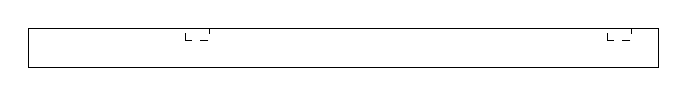
\begin{tikzpicture}[scale=0.2]
   \draw (0,0) rectangle (40,2.5);
   \draw [dashed] (10,1.7) rectangle (11.5,2.5);
   \draw [dashed] (36.8,1.7) rectangle (38.3,2.5);
   \dimline[line style={line width=0.5},extension start length=0.07,extension end length=0.07]{(11.5,4)}{(36.8,4)}{25.3 cm};
   \dimline[line style={line width=0.5},extension start length=-0.05,extension end length=-0.05]{(0,-1.5)}{(40,-1.5)}{40 cm};
  \end{tikzpicture}
 \end{center}
 \caption{(From top to bottom) Top view and front view of the X-axis segment with dimensions represented on a $1:5$ scale}
 \label{fig:xaxis}
\end{figure}

Following page shows the structure of the Y - axis segment which has a similar scheme of construction but with slightly reduced dimensions. \pagebreak

\begin{figure}[h]
 \begin{center}
  \begin{tikzpicture}[scale=0.2]
   \draw (0,0) rectangle (8.5,40);
   \draw [dashed] (0,6.7) rectangle (8.5,8.2);
   \draw [dashed] (0,30.5) rectangle (8.5,32);
   \hspace{-15mm}
   \dimline [extension start length=0.25, extension end length=0.25, line style = {line width=0.5}]{(0,0)}{(0,40)}{40 cm};
   \hspace{15mm}
   \dimline[line style={line width=0.5},extension start length=1,extension end length=1]{(0,42)}{(8.5,42)}{8.5 cm};
   \dimline[line style={line width=0.5},extension start length=0.3,extension end length=0.3]{(12,40)}{(12,32)}{8 cm};
   \dimline[line style={line width=0.5},extension start length=0.3,extension end length=0.3]{(12,30.5)}{(12,8.2)}{22.3 cm};
  \end{tikzpicture}
 \end{center}
 \begin{center}
  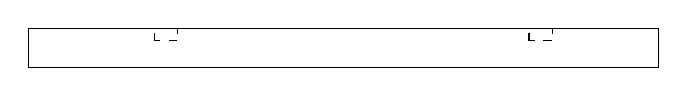
\begin{tikzpicture}[scale=0.2]
   \draw (0,0) rectangle (40,2.5);
   \draw [dashed] (8,1.7) rectangle (9.5,2.5);
   \draw [dashed] (31.8,1.7) rectangle (33.3,2.5);
   \dimline[line style={line width=0.5},extension start length=0.07,extension end length=0.07]{(9.5,4)}{(31.8,4)}{22.3 cm};
   \dimline[line style={line width=0.5},extension start length=-0.05,extension end length=-0.05]{(0,-1.5)}{(40,-1.5)}{40 cm};
  \end{tikzpicture}
 \end{center}
 \caption{(From top to bottom) Top view and front view of the Y-axis segment with dimensions represented on a $1:5$ scale}
 \label{fig:yaxis}
\end{figure}

The motor resides behind one block (say $B_{1}$) while the block on the other end is idle (say $B_{2}$). The face of $B_{1}$ which faces $B_{2}$ has two holes drilled in it. The guide rod connected to the motor shaft is inserted into the larger hole while the support rod is inserted into the smaller hole. The respective dimensions of the hole are clearly mentioned in the diagram and are identical for both $B_{1}$ and $B_{2}$. \par

Additionally as mentioned before dimension buffers are always necessary. The buffer which has been used here (both for $B_{1}$ and $B_{2}$) is: the center of the smaller hole is located at a distance of 1.5 cm from the left end while the center of the larger hole is 3 cm from the right end. The overall buffer which was available at the end for the two blocks were
(Left buffer $-$ radius of smaller hole) $+$ (Right buffer $-$ radius of larger hole)
$= (1.5 - 0.6) + (3 - 1.65)
 = 0.9 + 1.35
 = 2.25$ cm \par

The block $B_{2}$ as mentioned earlier is idle - the face of the block which does not face $B_{1}$ is fully empty. And the sole purpose of $B_{2}$ is to stabilise other ends of the main guide rod as well as the support rod. This is accomplished by the bearing arrangements made on the face facing the concerned face of $B_{1}$ as mentioned earlier. Details of the bearing design and the means through which they become compatible with the wooden block faces and the concerned guide or support rods are mentioned in the subsequent sections.

\begin{figure}[h]

 \begin{subfigure}{0.5\textwidth}
  \hspace{8mm}
  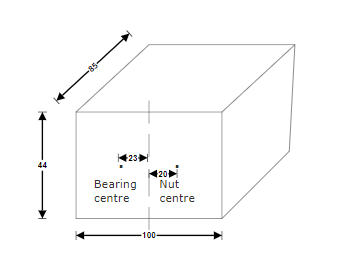
\includegraphics[width=0.8\linewidth, height=6cm]{Chapter_3/B1.png}
  \caption{Block $B_{1}$}
  \label{fig:b1}
 \end{subfigure}
 \begin{subfigure}{0.5\textwidth}
  \hspace{8mm}
  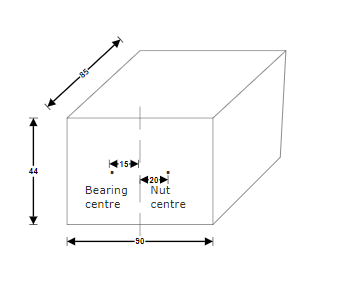
\includegraphics[width=0.8\linewidth, height=6cm]{Chapter_3/B2.png}
  \caption{Block $B_{2}$}
  \label{fig:b2}
 \end{subfigure}

 \caption{Three - dimensional representation of wooden blocks $B_{1}$ and $B_{2}$ with all the relevant dimensions and annotations (not to scale)}
 \label{fig:b1b2}
\end{figure}


\section{Guide rod and complementary support rods}

A pair of guide rod and complementary support rods are required for the XY axes. Before proceeding further it should be noted that the guide rod is threaded while the support rod is smooth. The threaded rod is made up of mild steel while the smooth rod material is stainless steel. As per design specifications, these rods must run perfectly parallel to each other. Ensuring the same is a critical design challenge. \par

The length of the threaded rod for the X- axis segment is 30 cm while for the Y- axis it comes out to be 27.5 cm. Further, there is no proper specification for the smooth rod lengths rather a larger sized ready made rod is cut to a length so that it fits between the blocks $B_{1}$ and $B_{2}$ (with all other dimensions taken into consideration). \par

However, although the rod (threaded) lengths are non identical, the thread pitch, the hole (to be drilled on the motor shaft end) specifications and the diameter are exactly identical. The thread pitch was decided at 1.25 mm. Since the rod on both ends will be held by smooth bearings, some part of the threading on both ends need to be removed. From the shaft side the threading has been deprecated by 3.3 cm while on the other end the threading has been reduced by 1.3 cm. The original diameter of the threaded rod was 1.2 cm however due to the thread deprivation on both sides the diameter has reduced to 1.0 cm on both ends for the concerned amount of thread deprived lengths. For the hole on the shaft side: the drill depth must be exactly equal to the shaft length with zero buffer. The shaft length is 2.3 cm and hence it is the drill depth as well. The diameter of the drill hole is fixed at 5 mm. Another hole must be drilled perpendicular to the rod axis at a distance of 1 cm from the shaft end. A fastening screw shall pass through this hole intersecting the motor shaft axis at a right angle.

% Show to scale image of the guide rod and complementary support rods one below the other %


\section{Bearing design}

As stated in the previous section it is obvious that a total of four bearings are needed: one on both ends of threaded rods of both the axes. Metal bearings in the manufacturing industry are specified by their inner diameters. Small spherical balls line up the space between the inner diameter and the outer diameters. These spherical balls reduce friction while the threaded rod rotates under the actuating action of the motor. These spherical balls are the actual bearings where the name of this machine part has come from. \par

In our project the inner diameter of the bearing is 1.0 cm (matching with the thread deprived rod diameter as mentioned in the previous section) while the outer diameter of the same comes out to be 3.3 cm.

\begin{figure}[h]
 \centering
 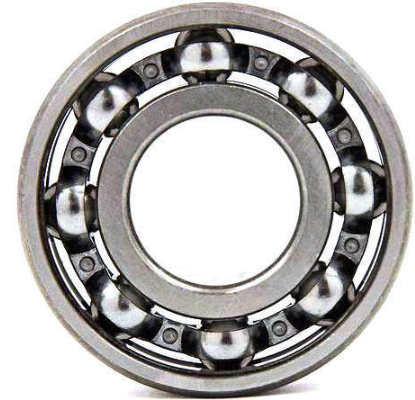
\includegraphics[scale = 0.5]{Chapter_3/bearing.PNG}
 \caption{Metal bearings similar to the ones used in the project}
 \label{fig:bearing}
\end{figure}

\section{Roller wheel section}

One end of the Y-axis (Wooden structure) is rested on top of the X-axis, while the other end is freely hanging. This might cause the Y-axis to lean towards that end. In order to make sure that the axis is stable, we have used a “ball castor wheel” which is attached to the free end of the Y-axis. This helps the axis to be perpendicularly aligned with X-axis and aligned in parallel with the base. To attach the wheel to the Y-axis we have made a wooden block which is of sufficient height to align the axis parallel to the base.

\begin{figure}[h]
 \centering
 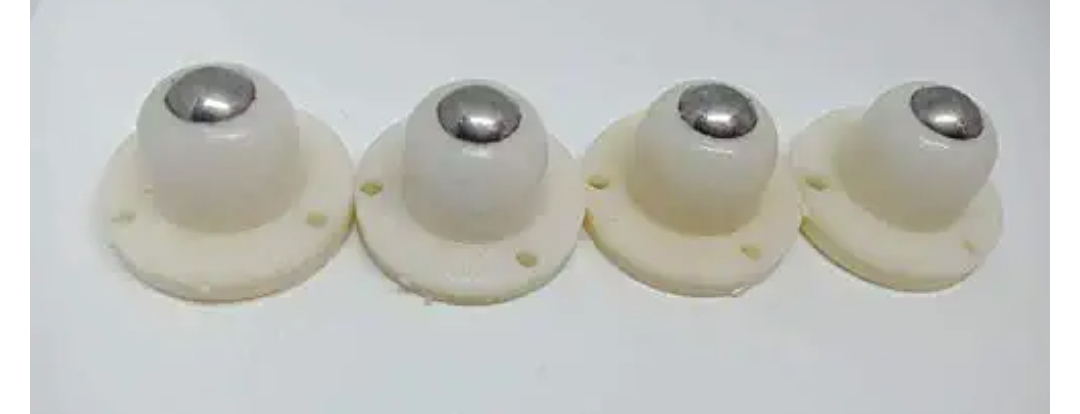
\includegraphics[scale = 0.32]{Chapter_3/ball_castor.jpeg}
 \caption{A set of castor wheels with a rubber endings similar to the one used in the project}
 \label{fig:ballcastor}
\end{figure}

\section{Engraving bits' selection}

The most important part of the CNC machine is the tooltip and its material constituents. The tooltip in case of our CNC machine is an engraving bit made of Tungsten Carbide. In general, such bits are expensive for either engraving or drilling applications. However, they are quite invaluable and universal in nature for almost all CNC based applications. For a CNC based PCB milling machine, a lot of attention is paid on the dimensions of the engraving bit because it directly corresponds to the accuracy of the system. For PCB milling purposes the minimum dimensions of the engraving bit that was purchased were 0.7 mm while the largest measured at about 3.2 mm. Following is an illustration of an engraving bit with all the relevant dimensions that would help the designer choose an appropriate size for a given set of specifications.

\begin{figure}[h]
 \centering
 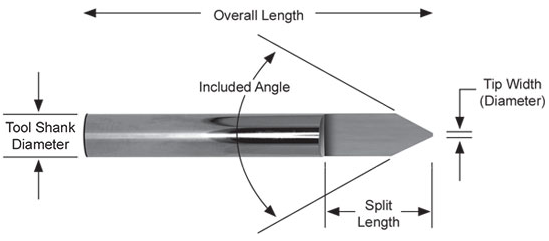
\includegraphics[scale = 0.75]{Chapter_3/engrav_bit.PNG}
 \caption{An illustration of a Tungsten Carbide engraving bit with all the relevant dimensions}
 \label{fig:ebit}
\end{figure}

\section{Coupling and fastening screws} \label{screws}
These two types of screws are required in abundance throughout the mechanical assembly for either fixing components to their respective base(s) of different materials OR to join/fix simultaneously actuated (usually) components. Now the primary parameter deciding screw specifications is material thickness on which the screw shall impinge. \par

For fastening screws impinging on the base or the plank material 1.5 mm screws are sufficient. For coupling screws, used only in one application: secure coupling of threaded rod and motor shaft, a specification of 3 mm is sufficient.

\begin{figure}[h]
 \centering
 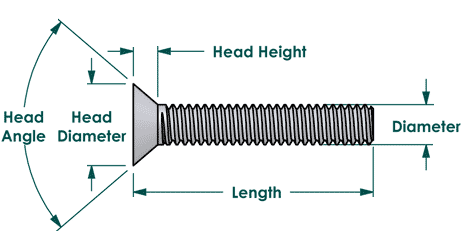
\includegraphics[scale = 0.59]{Chapter_3/coupling_screw.png}
 \caption{A coupling screw with all the relevant dimensions and similar to the ones used in the project}
 \label{fig:cscrew}
\end{figure} \pagebreak

\begin{figure}[h]
 \centering
 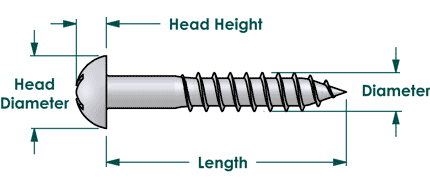
\includegraphics[scale = 0.59]{Chapter_3/fastening_screw.png}
 \caption{A fastening screw with all the relevant dimensions and similar to the ones used in the project}
 \label{fig:fscrew}
\end{figure}
